\documentclass[conference]{IEEEtran}

% ====== Idioma e codificacao (relatorio em portugues) ======
\usepackage[T1]{fontenc}
\usepackage[utf8]{inputenc}
% Hifenizacao PT-BR: descomente se seu TeX tiver o pacote (ex.: Overleaf).
%\usepackage[brazil]{babel}

\usepackage{float}
% ====== Figuras ======
\usepackage{graphicx}
\graphicspath{{figures/}}
\DeclareGraphicsExtensions{.pdf,.png,.jpg,.jpeg}

% ====== Matematica, tabelas, listas e links ======
\usepackage{amsmath}
\usepackage{amssymb}
\usepackage{array}
\usepackage{booktabs}
% \usepackage{algorithmic}   % descomente para escrever pseudocodigo
\usepackage{url}
\usepackage[hidelinks]{hyperref}
\raggedbottom

\begin{document}

\title{RideSmart: Modelagem e Análise de Rotas Urbanas com Grafos}

\author{
    \IEEEauthorblockN{\small Edivelton Rafaett Silva de Araújo}
    \IEEEauthorblockA{\scriptsize
        \textit{Departamento de Computação e Automação}\\
        \textit{Universidade Federal do Rio Grande do Norte}\\
        Natal, RN, Brasil\\
        Edivelton.rafaett.120@ufrn.edu.br}
    \and
    \IEEEauthorblockN{\small Francisco Micarlos Teixeira Pinto}
    \IEEEauthorblockA{\scriptsize
        \textit{Departamento de Computação e Automação}\\
        \textit{Universidade Federal do Rio Grande do Norte}\\
        Natal, RN, Brasil\\
        micarlos.teixeira.123@ufrn.edu.br}
    \and
    \IEEEauthorblockN{\small Joanderson Luan da Silva Linhares}
    \IEEEauthorblockA{\scriptsize
        \textit{Departamento de Computação e Automação}\\
        \textit{Universidade Federal do Rio Grande do Norte}\\
        Natal, RN, Brasil\\
        joanderson.linhares.701@ufrn.edu.br}
}

\maketitle

% =====================================================================
\section{Introdução}
% =====================================================================
Aplicativos de mobilidade urbana, como serviços de transporte por aplicativo, precisam constantemente decidir o melhor ponto de encontro entre o passageiro e o veículo. Muitas vezes, caminhar alguns metros até uma via de tráfego mais rápido pode reduzir o tempo total da viagem, evitando trechos congestionados ou de difícil acesso.

Formalmente, dados um ponto de origem $A$, um destino $B$ e uma distância máxima de caminhada $X$, busca-se um ponto de embarque $P$, localizado a, no máximo, $X$ metros a pé de $A$, que minimize o custo total da viagem. A rota é decomposta em dois trechos: $A \to P$, percorrido a pé, e $P \to B$, percorrido de carro. O caso sem caminhada, em que $P = A$, serve como referência para medir o ganho obtido.

As contribuições deste relatório são: (i) a modelagem do problema sobre grafos reais de uma cidade; (ii) a comparação de quatro algoritmos de caminho mínimo quanto à eficiência e à qualidade da solução; (iii) a análise do impacto de um trânsito sintético; e (iv) a discussão do trade-off entre caminhar e chegar mais rápido. O restante do relatório está organizado da seguinte forma: a Seção II apresenta a modelagem do problema; a Seção III descreve os algoritmos utilizados; a Seção IV detalha os experimentos; a Seção V apresenta os resultados; a Seção VI discute criticamente os resultados obtidos; e, por fim, a Seção VII apresenta as conclusões.

% =====================================================================
\section{Modelagem do Problema}
% =====================================================================
\subsection{Representação da malha urbana em dois grafos}
A cidade foi representada por dois grafos distintos obtidos do OpenStreetMap com a biblioteca OSMnx: um grafo de pedestres $G_{walk}$, definido por \texttt{network\_type="walk"}, e um grafo de veículos $G_{drive}$, definido por \texttt{network\_type="drive"}. A separação é importante pois pedestres e carros não compartilham exatamente a mesma malha urbana. Usar um único grafo poderia permitir que o carro trafegasse por vias exclusivas de pedestres ou, no caso contrário, obrigaria o pedestre a seguir apenas ruas destinadas a veículos.

Assim, o trecho $A \to P$ é resolvido em $G_{walk}$, enquanto o trecho $P \to B$ é resolvido em $G_{drive}$. Nos grafos, os nós representam interseções e extremidades de vias, e as arestas representam os segmentos de rua ou calçada que as conectam. O grafo de veículos é direcionado, respeitando o sentido de mão e contramão das vias.

\subsection{Pontos de origem e destino}
O ponto de origem $A$ corresponde à calçada em frente ao IFRN -- Campus Natal Central, nas coordenadas $(-5{,}811677,\ -35{,}204526)$. O ponto de destino $B$ é o estabelecimento Agaé, fornecido por endereço textual e geocodificado pelo OSMnx em $(-5{,}840552,\ -35{,}211156)$.

Cada ponto é mapeado para o nó mais próximo em cada grafo. Como o nó de caminhada de $A$ não existe na malha viária, ele foi associado ao nó de carro mais próximo, a $13{,}57$ m de distância. Essa distância foi registrada apenas como aproximação espacial. O destino $B$ utilizado pelo carro corresponde ao nó mais próximo na malha \texttt{drive}.

\subsection{Pesos das arestas}
Cada aresta possui três pesos principais. O peso \texttt{length} representa o comprimento físico da aresta, em metros. O peso \texttt{travel\_time} representa o tempo de deslocamento, em segundos, sem congestionamento, estimado a partir das velocidades atribuídas pelo OSMnx:
\begin{equation}
\texttt{travel\_time} = \frac{\texttt{length}}{v_{via}}.
\end{equation}
O peso \texttt{traffic\_time} representa o tempo de deslocamento sob trânsito sintético:
\begin{equation}
\texttt{traffic\_time} = \texttt{travel\_time} \times f,
\end{equation}
em que $f \in [2,4]$ nas arestas penalizadas e $f = 1$ nas demais. O trecho a pé é convertido em tempo considerando uma velocidade de caminhada de $5$ km/h.

\subsection{Geração e validação dos candidatos $P$}
O ponto $P$ não é escolhido manualmente. Primeiro, são enumerados todos os nós alcançáveis a pé a partir de $A$ dentro do raio $X$, isto é, aqueles que satisfazem:
\begin{equation}
D_{walk}(A,P) \leq X.
\end{equation}
Em seguida, cada candidato é associado à malha viária por uma regra em duas etapas. Se o mesmo nó existir em $G_{drive}$, ele é usado diretamente. Caso contrário, utiliza-se o nó viário mais próximo, desde que esteja a, no máximo, $25$ m de distância. Essa pequena distância de aproximação é somada ao custo de caminhada.

No cenário avaliado, ilustrado na Figura~\ref{fig:mapa}, $224$ nós eram alcançáveis a pé e $77$ foram considerados válidos para embarque. Destes, $41$ eram nós compartilhados entre as malhas e $183$ foram associados ao nó viário mais próximo.

\begin{figure}[H] \centering 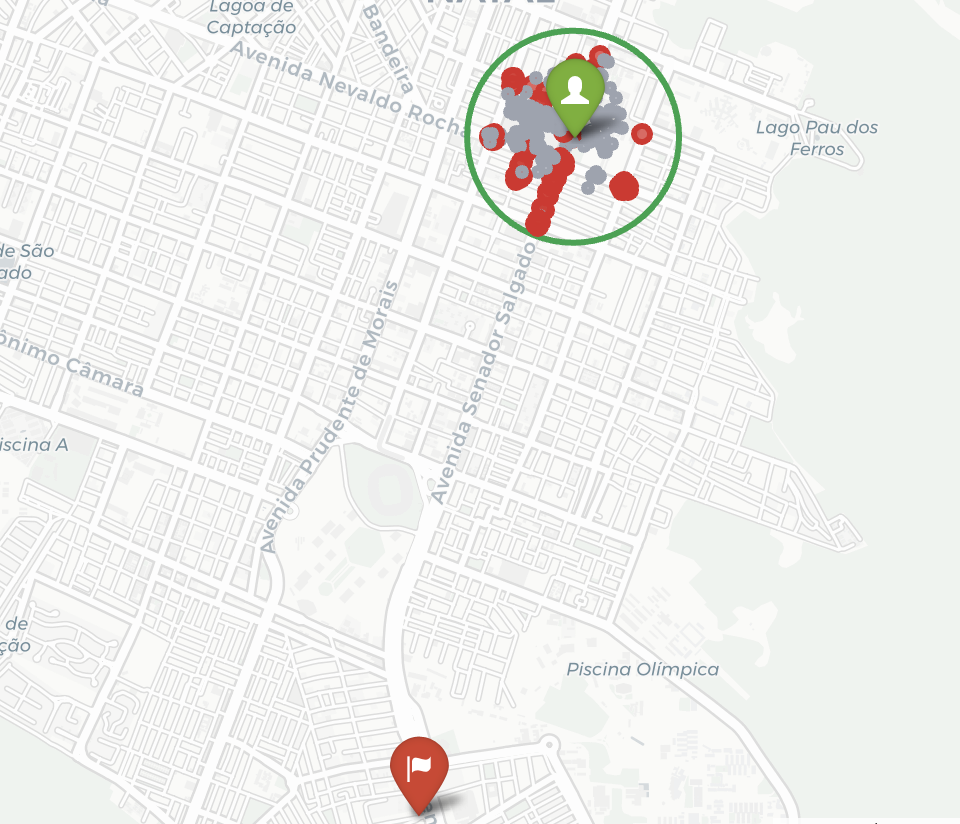
\includegraphics[width=0.80\columnwidth]{01_mapa_cenario.png} \caption{Cenário em Natal/RN: origem $A$ em verde, destino $B$ indicado pela bandeira, raio de caminhada $X$ e candidatos a ponto de embarque $P$.} \label{fig:mapa} \end{figure}

\subsection{Função de custo e caso de referência}
O custo de uma solução depende do critério utilizado. Para distância, tem-se:
\begin{equation}
\text{Custo}_D(P) = D_{walk}(A,P) + D_{drive}(P,B).
\end{equation}
Para tempo, tem-se:
\begin{equation}
\text{Custo}_T(P) = T_{walk}(A,P) + T_{drive}(P,B),
\end{equation}
em que $T_{drive}$ usa \texttt{travel\_time} ou \texttt{traffic\_time}, conforme o cenário analisado. O caso sem caminhada corresponde a $P = A$ e serve como base para o cálculo do ganho.

% =====================================================================
\section{Algoritmos Utilizados}
% =====================================================================
Foram implementados e comparados quatro algoritmos de caminho mínimo, todos avaliados ponto a ponto, isto é, uma busca $P_i \to B$ para cada candidato. Dessa forma, a contagem de nós expandidos permanece comparável entre os métodos.

\textbf{Dijkstra simples.} Versão base do algoritmo, sem uso de fila de prioridade. A cada iteração, o nó aberto de menor custo é escolhido por busca linear. Essa abordagem serve como linha de base didática para comparação com as versões mais eficientes.

\textbf{Dijkstra com heap.} Mantém a mesma lógica de relaxamento das arestas, mas a seleção do próximo nó é feita com uma fila de prioridade, implementada com \texttt{heapq}. Com isso, evita-se a varredura linear dos nós abertos. Em grafos urbanos esparsos, essa estratégia tende a reduzir o tempo de execução.

\textbf{A*.} Busca informada que utiliza a função de avaliação $f(n) = g(n) + h(n)$, em que $g(n)$ representa o custo real acumulado até o nó atual e $h(n)$ representa uma heurística admissível. Neste trabalho, a heurística utilizada é a distância em linha reta até o destino, convertida em tempo por uma velocidade máxima estimada quando o critério analisado é temporal.

\textbf{Dijkstra bidirecional.} Executa duas buscas simultâneas: uma a partir da origem e outra a partir do destino, esta última sobre o grafo reverso. Quando as buscas se encontram, o caminho é reconstruído. Essa abordagem representa uma alternativa eficiente para consultas ponto a ponto em grafos.

% =====================================================================
\section{Experimentos}
% =====================================================================
O cenário avaliado vai da calçada do IFRN -- Campus Natal Central, representada por $A$, até o Agaé, representado por $B$, com raio de caminhada $X = 500$ m. A Tabela~\ref{tab:parametros} resume os principais parâmetros do experimento e a dimensão dos grafos.

\begin{table}[H] \centering \caption{Parâmetros do experimento} \label{tab:parametros} \footnotesize \begin{tabular}{@{}ll@{}} \toprule Parâmetro & Valor \\ \midrule Cidade & Natal/RN \\ Raio de caminhada $X$ & 500 m \\ Velocidade a pé & 5 km/h \\ Distância máxima entre $P$ e o nó de carro & 25 m \\ Semente aleatória & 42 \\ Grafo de caminhada & 26.728 nós / 78.120 arestas \\ Grafo de direção & 18.578 nós / 48.183 arestas \\ Candidatos alcançáveis / válidos & 224 / 77 \\ \bottomrule \end{tabular} \end{table}

O trânsito sintético foi construído de forma controlada. Primeiro, calcularam-se as rotas mais rápidas sem trânsito para todos os algoritmos. Em seguida, os trechos dessas rotas foram reunidos em um conjunto único, do qual $14$ arestas foram penalizadas. Esse número corresponde a uma proporção de $0{,}35$ dos pares únicos, com fator de penalização entre $2$ e $4$ e semente fixa para garantir reprodutibilidade.

Penalizar rotas que já eram boas, em vez de escolher ruas aleatórias, torna a comparação mais fiel ao problema analisado. Além disso, o mesmo peso \texttt{traffic\_time} é aplicado a todos os algoritmos, garantindo que as comparações sejam feitas sob as mesmas condições. As métricas coletadas foram o custo total da viagem, o número de nós expandidos, o tempo de execução e o ganho em relação ao caso sem caminhada.

% =====================================================================
\section{Resultados}
% =====================================================================
\subsection{Ganho ao caminhar até o ponto $P$}

A Tabela~\ref{tab:ganho} apresenta o ganho obtido ao permitir caminhada nos três critérios. Em todos eles, o ganho foi positivo, ou seja, caminhar reduziu o custo da viagem. No critério de distância, o melhor ponto foi $P_{143}$: a viagem caiu de $4.456{,}30$ m, sem caminhada, para $3.439{,}09$ m, uma economia de $1.017{,}21$ m, equivalente a $22{,}8\%$, ao custo de uma caminhada de $454{,}32$ m, aproximadamente $5{,}5$ min. No critério de tempo sem trânsito, o melhor ponto foi $P_4$: o tempo caiu de $242{,}11$ s para $197{,}88$ s, uma economia de $44{,}23$ s, equivalente a $18{,}3\%$, com uma caminhada de apenas $33{,}83$ m, aproximadamente $0{,}4$ min. Com trânsito sintético, o mesmo $P_4$ economizou $63{,}51$ s, equivalente a $18{,}9\%$.

\begin{table}[H]
    \centering
    \caption{Ganho ao caminhar até o ponto $P$}
    \label{tab:ganho}
    \footnotesize
    \resizebox{\columnwidth}{!}{%
    \begin{tabular}{@{}lccccc@{}}
        \toprule
        Critério & $P$ & Custo c/ $P$ & Custo s/ cam. & Ganho & \% \\
        \midrule
        Menor distância   & $P_{143}$ & $3.439{,}09$ m & $4.456{,}30$ m & $1.017{,}21$ m & $22{,}8$ \\
        Tempo s/ trânsito & $P_4$     & $197{,}88$ s   & $242{,}11$ s   & $44{,}23$ s    & $18{,}3$ \\
        Tempo c/ trânsito & $P_4$     & $273{,}30$ s   & $336{,}81$ s   & $63{,}51$ s    & $18{,}9$ \\
        \bottomrule
    \end{tabular}%
    }
\end{table}

\subsection{Menor distância não é a rota mais rápida}

Os critérios escolheram pontos de embarque diferentes. A menor distância usa $P_{143}$, que exige $454$ m a pé, enquanto a rota mais rápida usa $P_4$, com apenas $34$ m a pé. A explicação é que minimizar metros e minimizar segundos são objetivos distintos: o ponto que encurta o trajeto físico exige uma caminhada longa, prejudicando o tempo total, enquanto a rota mais rápida prefere caminhar pouco e embarcar em uma via mais veloz.

\subsection{Efeito do trânsito sintético}

O congestionamento penalizou mais a rota sem caminhada do que a rota com embarque em $P$. Sem trânsito, a rota direta $A \to B$ percorria $4.456{,}30$ m em $242{,}11$ s. Com trânsito, o carro desviou para um caminho mais longo, de $4.915{,}22$ m, elevando o tempo para $336{,}81$ s. Já a rota com embarque em $P_4$ manteve o mesmo trajeto físico, de $3.441{,}51$ m, com o tempo subindo de $173{,}52$ s para $248{,}94$ s. Assim, o ganho da caminhada aumentou de $44{,}23$ s para $63{,}51$ s quando o trânsito entrou em cena.

\subsection{Eficiência da busca: nós expandidos}

A Figura~\ref{fig:nos} e a Tabela~\ref{tab:perf} mostram o esforço de busca. No critério de distância, o A* expandiu apenas $13.025$ nós, contra $255.521$ dos dois Dijkstras, uma redução de aproximadamente $95\%$, e $116.261$ do bidirecional. No critério de tempo sem trânsito, o padrão se repete: $8.291$ nós para o A*, $146.859$ para os Dijkstras e $46.413$ para o bidirecional. A heurística geográfica direcionou a busca para o destino, em vez de espalhá-la uniformemente pela malha.

\begin{figure}[H]
    \centering
    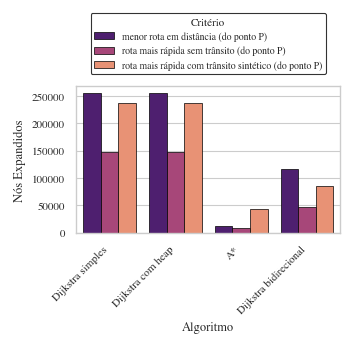
\includegraphics[width=0.80\columnwidth]{chart_nos_expandidos.png}
    \caption{Nós expandidos por algoritmo e critério de avaliação.}
    \label{fig:nos}
\end{figure}

\begin{table}[H]
    \centering
    \caption{Desempenho computacional no critério de distância, com caminhada}
    \label{tab:perf}
    \footnotesize
    \resizebox{\columnwidth}{!}{%
    \begin{tabular}{@{}lrr@{}}
        \toprule
        Algoritmo & Nós expandidos & Tempo (ms) \\
        \midrule
        Dijkstra simples      & $255.521$ & $13.864{,}21$ \\
        Dijkstra com heap     & $255.521$ & $773{,}97$ \\
        A*                    & $13.025$  & $101{,}55$ \\
        Dijkstra bidirecional & $116.261$ & $343{,}43$ \\
        \bottomrule
    \end{tabular}%
    }
\end{table}

\subsection{Tempo de execução}

A Figura~\ref{fig:tempo} apresenta o tempo de execução. Embora os dois Dijkstras expandam exatamente o mesmo número de nós, o Dijkstra com heap foi cerca de $18\times$ mais rápido que o simples no critério de distância, com $773{,}97$ ms contra $13.864{,}21$ ms, e cerca de $10\times$ mais rápido no critério de tempo, com $460{,}51$ ms contra $4.776{,}83$ ms, graças à fila de prioridade. O A* foi o mais rápido de todos, com $101{,}55$ ms na distância e $56{,}62$ ms no tempo, enquanto o bidirecional ficou em posição intermediária, com $343{,}43$ ms e $146{,}24$ ms.

\begin{figure}[H]
    \centering
    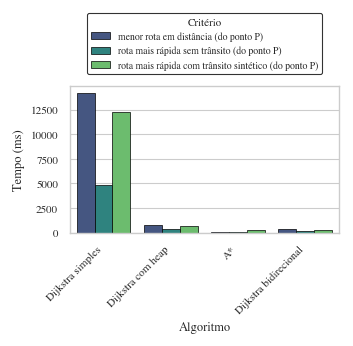
\includegraphics[width=0.80\columnwidth]{chart_tempo_execucao.png}
    \caption{Tempo de execução em milissegundos por algoritmo e critério.}
    \label{fig:tempo}
\end{figure}

\subsection{Decomposição do tempo total de viagem}

A Figura~\ref{fig:impacto} decompõe o tempo total da viagem com o A*. Sem trânsito, a viagem cai de $4{,}0$ min, considerando o trajeto completo de carro, para $3{,}3$ min ao usar o ponto $P$, dos quais $2{,}9$ min são de carro e $0{,}4$ min de caminhada. Com trânsito sintético, a viagem cai de $5{,}6$ min para $4{,}6$ min, sendo $4{,}2$ min de carro e $0{,}4$ min de caminhada. A figura evidencia que a combinação de caminhada curta com transporte motorizado reduz o tempo total nos dois cenários, e que o ganho é maior sob congestionamento.

\begin{figure}[H]
    \centering
    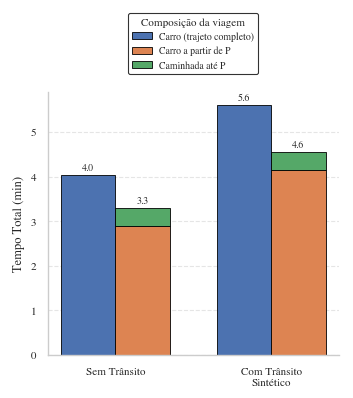
\includegraphics[width=0.80\columnwidth]{chart_impacto_caminhada.png}
    \caption{Impacto da caminhada no tempo total de viagem, sem e com trânsito.}
    \label{fig:impacto}
\end{figure}

% =====================================================================
\section{Discussão}
% =====================================================================

Neste cenário, caminhar compensou em todos os critérios. Em particular, no critério de tempo, uma caminhada de poucos metros já reposicionou o embarque em uma via mais rápida. Ainda assim, caminhar nem sempre ajuda: quando $A$ já está sobre uma via boa, quando $X$ é pequeno demais para alcançar uma via vantajosa, ou quando se otimiza o tempo, mas o melhor ponto em distância exige uma caminhada longa, o caso sem caminhada pode ser preferível.

O A* destacou-se em eficiência sem abrir mão da otimalidade, pois sua heurística é admissível. Um ponto a se observar é que o Dijkstra bidirecional escolheu $P_{15}$, com $3.440{,}90$ m, em vez de $P_{143}$, com $3.439{,}09$ m, no critério de distância. A diferença é de apenas $1{,}8$ m, equivalente a $0{,}05\%$, provavelmente devido à condição de parada e à reconstrução no ponto de encontro das duas buscas.

A modelagem possui limitações: o trânsito é sintético e não reflete fluxo real; as velocidades são estimativas padrão, sem semáforos ou conversões; não há posição inicial do veículo antes do embarque; o embarque é aproximado por um limite de $25$ m; a velocidade de caminhada é fixa; cada critério é otimizado isoladamente; e foi avaliado um único par origem--destino.

% =====================================================================
\section{Conclusão}
% =====================================================================
Este relatório modelou a escolha do ponto de embarque como um problema de caminho mínimo sobre grafos reais e mostrou que permitir uma caminhada curta melhorou a viagem em até $22{,}8\%$ em distância e cerca de $18$ a $19\%$ em tempo. Entre os algoritmos, o A* foi o mais eficiente, expandindo $\approx 95\%$ menos nós que o Dijkstra, e o Dijkstra com heap foi cerca de $18\times$ mais rápido que o simples. 

\end{document}
